\documentclass[]{article}

\usepackage[l2tabu, orthodox]{nag}


% % % % % % % % % %
% MATH
% % % % % % % % % %
\usepackage[fleqn]{amsmath}	% fleqn for left alignment of math blocks (as in classicthesis)
\usepackage{amssymb}
\newcommand{\eq}[1]{\begin{align*}#1\end{align*}}
\newcommand\numberthis{\addtocounter{equation}{1}\tag{\theequation}}


% % % % % % % % % %
% FONTS
% % % % % % % % % %
\usepackage[osf,sc]{mathpazo} % Palatino as the main font
\linespread{1.05}\selectfont % Palatino needs some extra spacing, here 5% extra
%\usepackage[scaled=0.85]{beramono}
\usepackage[euler-digits]{eulervm} % nicer math font


% % % % % % % % % %
% FLOATS, FIGURAES, AND TABLES
% % % % % % % % % %
\usepackage{graphicx} 		% Required for including images
\usepackage{caption}
\captionsetup{font=small} 	% format=hang,
\usepackage{subfig}
\usepackage{tabularx}
\setlength{\extrarowheight}{3pt} % increase table row height
\usepackage{pbox} 			% for linebreaking in cells
\usepackage{multicol, multirow}
\usepackage{tikz}
\usetikzlibrary{fit,arrows,shapes}
\usetikzlibrary{decorations.pathreplacing}



% % % % % % % % % %
% BIBLIOGRAPY
% % % % % % % % % %


\usepackage[
	%backend=biber, %instead of bibtex
	backend=bibtex8,bibencoding=ascii,%
	language=auto,%
	style=numeric-comp,%
	%style=authoryear-comp, % Author 1999, 2010
	%bibstyle=authoryear,dashed=false, % dashed: substitute rep. author with ---
	sorting=nyt, % name, year, title
	maxbibnames=10, % default: 3, et al.
	%backref=true,%
	natbib=true % natbib compatibility mode (\citep and \citet still work)
]{biblatex}
\usepackage{biblatex}
% alternative: \usepackage{natbib}


% % % % % % % % % %
% MISC
% % % % % % % % % %
\usepackage
[
%disable
]{todonotes}
\usepackage[utf8]{inputenc} % allow utf-8 input
\usepackage[T1]{fontenc}    % use 8-bit T1 fonts
\usepackage[english]{babel} % hyphenation, special characters, ...
\usepackage{csquotes}		% recommended with babel for quotes
\usepackage{hyperref}       % hyperlinks
\usepackage{cleveref}		% provides \cref for nice in-document refs
\usepackage{url}            % simple URL typesetting
\usepackage{nicefrac}       % compact symbols for 1/2, etc.
\usepackage
[
activate={true,nocompatibility}, % activate protrusion and expansion
final,						% enable microtype; use "draft" to disable
tracking=true,
kerning=true,
spacing=true,
factor=1100,				% add 10% to the protrusion amount (default: 1000)
stretch=10,					% reduce stretchability (default: 20)
shrink=10					% reduce shrinkability (default: 20)
]
{microtype}
\usepackage{cancel}			% easy cancelling of terms: \cancel{expression}
\usepackage{mlmacros}

% needed for leftmargin ident of the description env
\usepackage{enumitem}

\usepackage{tikz}
\usetikzlibrary{arrows.meta}


%opening
\title{Predictive Coding Notes}
\author{Adam Kosiorek}


\variables{x,y,z}
\probdists{p,q}

\begin{document}

\maketitle

%\begin{abstract}
%
%\end{abstract}

%\newcommand{\encodeblock}[1]{ %inpt, layer_num
%	
%	\node[circle, draw] (delta_#1) at (0, 1) {$\Delta \b#1$};
%	\node[circle, draw] (hat_#1) at (-1, 1) {$\widehat{\bx}_1$};
%	\node[circle, draw] (z01) at (-2, 2) {$\bz_0^1$};
%	\node[circle, draw] (z11) at (0, 2) {$\bz_0^1$};
%	
%	\draw[->] (#1) to (delta_#1);
%	\draw[->] (hat_#1) to (delta_#1);
%	\draw[->] (z01) to (hat_#1);
%	\draw[->] (z01) to (z11);
%	\draw[->] (delta_#1) to (z11);
%	
%}
\section{Predictive Coding}

	Modern sequential predictive models tend to update its hidden state at every time-step. It can be argued, however, that if a model is able to predict the world perfectly, it should not update its state. On the contrary, if a perfect prediction is available, the model should also be capable of evolving its hidden state so as to reflect the change of the state of the world \wrt the prediction. Predictive coding formalises this behaviour by using only prediction errors to update the world. 
	
	The idea dates back to the Kalman filter and beyond\addref. Recent advances in neural networks make it possible to frame the predictive coding problem as an auto-regressive neural network. Indeed, it has been addressed in a number of papers \addref{cortexnet, prednet, some others}. These models use the mean-squared error between the prediction and the corresponding input to update their hidden state. It leads to an ill-posed problem since there are many futures possible. The prediction, which is a maximum-likelihood estimate of what might happen, is only a single instantiation thereof. It would be theoretically more sound to normalise prediction errors by the covariance matrix of errors, an approach adopted by Kalman filtering. Friston \addref{Friston} argues this is also the approach taken by the brain, and it explains a lot of phenomena happening there. He suggests that the computational architecture of the brain forms a hierarchical system, where each layer constantly predicts the output of the lower levels of hierarchy in a fully Bayesian fashion. It gives rise to surprise, which is the negative log-likelihood of the inputs under the predictive distribution of the model. Friston argues that surprise leads to error normalisation \wrt prediction uncertainty, which can be interpreted as attention.

	Free-energy minimisation problems can be often written as variational inference, which is also true in this case. In what follows, we specify the model as a variational autoencoder, show its computational graph and derive the variational lower bound.

\section{Variational Distribution}

	Let $\bxTs$ be a timeseries of observations\eg image sequence or a series of joint angles. The probability distribution over input sequences $\p{\bxTs}$ can be expressed by the product law as $\p{\bxTs}= \prod_{t=1}^T \p{\bxt}{\bx_{1:t-1}}$ and is in general intractable. We introduce a hierarchy of latent variables $\byTs$, where $\byt = \set{ \bzTs^l }_{l=1}^L$, such that the joint probability distribution $\p{\bxTs, \byTs}{}{\theta} = \p{\bxTs}{\byTs}{\theta}\p{\byTs}{}{\theta}$ lives in the space of parametric probability distributions parametrised by parameters $\theta$ and is tractable. We further assume the following factorisation:
	\begin{description}[leftmargin=\parindent]
		\item[prior] The prior distribution is a dynamical model of the latent space. It specifies the probability distribution over the initial states $\by_0$ and the transition probabilities between states. It may or may not be stationary.
		\begin{equation}
		\p{\by_{0:T-1}}{}{\theta} = \p{\by_0}{}{\theta} \prod_{t=1}^{T-1} \p{\byt}{\by_{t-1}}{\theta}
		\end{equation}
		
		\item[generating distribution] The generating distribution decodes the samples from the latent space back into the observation space. It uses the learnt dynamics model internally to propagate the state forward.
		\begin{equation}
			\begin{aligned}
				\p{\bxTs}{\byTs}{\theta} &= \int \p{\by_0}{}{\theta} \prod_{t=0}^T \p{\bx_{t+1}}{\byt}{\theta}\dint \by_0 \\
				&= \int \p{\by_0}{}{\theta} \prod_{t=0}^T \int \p{\bx_{t+1}}{\widehat{\by}_{t+1}}{\theta} \p{\widehat{\by}_{t+1}}{\byt}{\theta} \dint \widehat{\by}_{t+1} \dint \by_0 \\
				&= \p{\bxTs}{\by_{1:T-1}}{\theta}
			\end{aligned}
		\end{equation}
	
		\item[posterior distribution] The posterior distribution is intractable, although its general form reads as follows:
		\begin{equation}
			\p{\by_{1:T-1}}{\bx_{1:T-1}} = \int \prod_{t=1}^{T-1} \p{\byt}{\bxt, \by_{t-1}} \p{\by_0}{}{\theta} \dint \by_0
		\end{equation}
		
		\item[approximate posterior] We approximate the posterior with a tractable parametric distribution $\q{}{}{\phi}$ by assuming that the hidden state $\byt$ is Markovian.
		\begin{equation}
			\q{\by_{1:T-1}}{\bx_{1:T-1}, \by_0}{\phi} = \prod_{t=1}^{T-1} \q{\byt}{\bxt, \by_{t-1}}{\phi}
		\end{equation}
	\end{description}
	Moreover, since we learn the latent dynamics model, the generating model predicts the input at the next time-step as opposed to standard VAE practice, where it merely reconstructs the input from the current time-step.
	
	\subsection{Multimodal Distributions for Predictive Coding}
	
	The expressive power of VAEs is often constrained by too simple a form of the approximate posterior distribution and increasing the complexity of the approximate posterior typically leads to better results \addref{normalizing flows, inverse autoregressive flows, dvbf}. Complexity-increasing methods used so far typically lead to increased correlation between latent variables and/or multimodal distribution. While correlated latent variables may be desirable, they are against the principle coding principle \addref{is that even true?}, since the latent variables should be orthogonal in order to maximum the maximum amount of information possible. Multimodal distributions don't have this caveat. In case of predictive-coding, however, they lead to scenarios where the computed surprise on the input is ambiguous. 
	
	Assume a bimodal distribution predictive $\p{\widehat{z}_{t+1}}{\zt} = a \gauss{-1, 1} + b \gauss{1, 1}$ and an input $z_{t+1}$. The value of the surprise is $s_{t+1} = -\log \p{\widehat{z}_{t+1}}{\zt}\lvert_{\widehat{z}_{t+1} = z_{t+1}}$. Even in case of a unimodal distribution, there exist an infinite number of points giving rise to the same value of surprise, but at least that value exclusively determines the distance of the input from that mode. In case of a multimodal distribution, the value of surprise indicates the distance, but we don't know from which mode. That leads to encoding ambiguity and is disturbing. This in itself could be an argument of why all distributions used in predictive coding should be unimodal. Is that the case in the brain?
	
\section{ELBO}
	
	It's looking pretty straightforward, but to be derived...
	
\section{Architecture}

	We need $L$ encoders, $L$ decoders, $L$ dynamic models and $L-1$ combinators. Each of the components could in principle be either stochastic or deterministic. To contain the model within the VAE framework, we take stochastic encoders and decoders, stochastic dynamic models, which we use as latent space priors, and deterministic combinators. Computation graph is given in \cref{fig:comp}.
	\begin{description}[leftmargin=\parindent]
		\item[encoder] Given the previous latent state and a prediction error, it computes the parameters of the approximate posterior $\q{\bz_t^l}{\bz_{t-1}^l, \Delta \bz_t^l}{\phi}$.
		\item[dynamic model] Computes the probability distribution over the new state estimate given a a previous state estimate, it's part of the prior as $\p{\bz_{t+1}}{\bz_{t-1}}{\theta}$.
		\item[combinator] State is predicted based on more abstract representation. This module refines the prediction by using lower-level information available in the previous state estimate. It is a part of the generating model.
		\item[decoder] The final part of the generating model, transforms the refined state estimate computed by the combinator and computes the probability distribution over the lower level state estimate $\p{\bz_{t+1}^l}{ \bz_{t}^{l+1}, \widehat{\bz}_{t+1}^{l+1} }{\theta}$.
	\end{description}


	\begin{figure}
		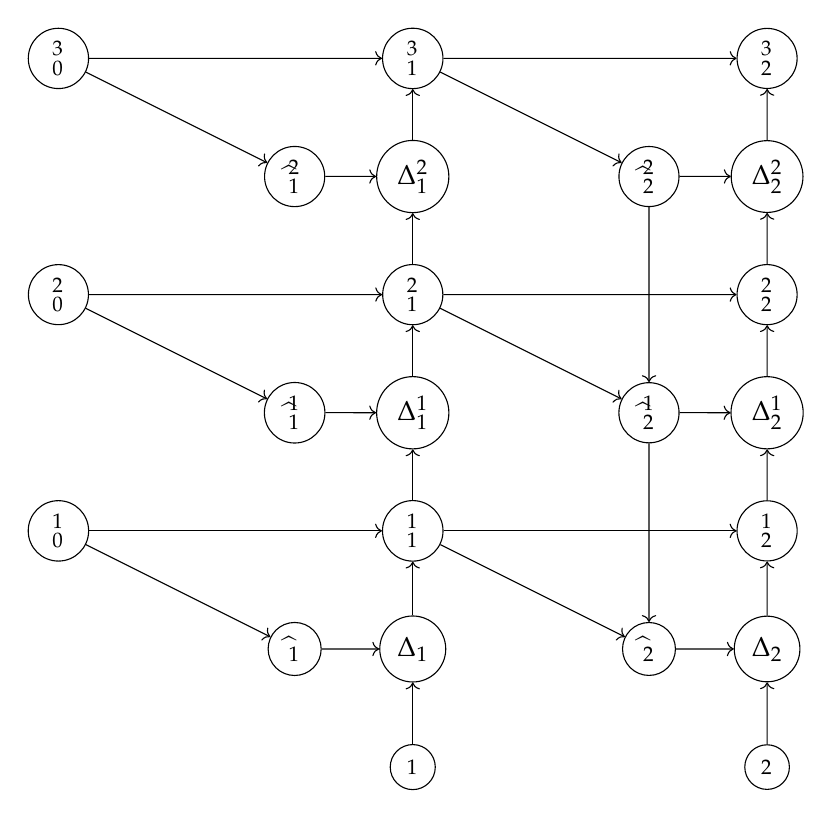
\begin{tikzpicture}[scale=1.5]
		
%			Input	$$$$$$$$$$$$$$$$$$$$$$$$$$$$$$$$$$$$$$$$$$$$$$$$$$$$$$$$$$
			\node[circle, draw] (x1) at (0, 0) {$\bx_1$};
%			\encodeblock{x_1}

%	Encoder $$$$$$$$$$$$$$$$$$$$$$$$$$$$$$$$$$$$$$$$$$$$$$$$$$$$$$$$$$$$
			\node[circle, draw] (delta_x1) at (0, 1) {$\Delta \bx_1$};
			\node[circle, draw] (hat_x1) at (-1, 1) {$\widehat{\bx}_1$};
			\node[circle, draw] (z01) at (-3, 2) {$\bz_0^1$};
			\node[circle, draw] (z11) at (0, 2) {$\bz_1^1$};
			
			\draw[->] (x1) to (delta_x1);
			\draw[->] (hat_x1) to (delta_x1);
			\draw[->] (z01) to (hat_x1);
			\draw[->] (z01) to (z11);
			\draw[->] (delta_x1) to (z11);
			
			\node[circle, draw] (delta_z11) at (0, 3) {$\Delta \bz_1^1$};
			\node[circle, draw] (hat_z11) at (-1, 3) {$\widehat{\bz}_1^1$};
			\node[circle, draw] (z02) at (-3, 4) {$\bz_0^2$};
			\node[circle, draw] (z12) at (0, 4) {$\bz_1^2$};
			
			\draw[->] (z11) to (delta_z11);
			\draw[->] (hat_z11) to (delta_z11);
			\draw[->] (z02) to (hat_z11);
			\draw[->] (z02) to (z12);
			\draw[->] (delta_z11) to (z12);
			
			\node[circle, draw] (delta_z12) at (0, 5) {$\Delta \bz_1^2$};
			\node[circle, draw] (hat_z12) at (-1, 5) {$\widehat{\bz}_1^2$};
			\node[circle, draw] (z03) at (-3, 6) {$\bz_0^3$};
			\node[circle, draw] (z13) at (0, 6) {$\bz_1^3$};
			
			\draw[->] (z12) to (delta_z12);
			\draw[->] (hat_z12) to (delta_z12);
			\draw[->] (z03) to (hat_z12);
			\draw[->] (z03) to (z13);
			\draw[->] (delta_z12) to (z13);

%			Decoder	$$$$$$$$$$$$$$$$$$$$$$$$$$$$$$$$$$$$$$$$$$$$$$$$$$$$$$$$$$$

		\node[circle, draw] (z23) at (3, 6) {$\bz_2^3$};
		\node[circle, draw] (hat_z22) at (2, 5) {$\widehat{\bz}_2^2$};
		\node[circle, draw] (delta_z22) at (3, 5) {$\Delta \bz_2^2$};
		
		\draw[->] (z13) to (z23);
		\draw[->] (z13) to (hat_z22);
		\draw[->] (hat_z22) to (delta_z22);
		\draw[->] (delta_z22) to (z23);
		
		
		\node[circle, draw] (z22) at (3, 4) {$\bz_2^2$};
		\node[circle, draw] (hat_z21) at (2, 3) {$\widehat{\bz}_2^1$};
		\node[circle, draw] (delta_z21) at (3, 3) {$\Delta \bz_2^1$};
		
		\draw[->] (z12) to (z22);
		\draw[->] (z12) to (hat_z21);
		\draw[->] (hat_z21) to (delta_z21);
		\draw[->] (delta_z21) to (z22);
		
		\draw[->] (z22) to (delta_z22);
		\draw[->] (hat_z22) to (hat_z21);
		
		
		
		\node[circle, draw] (z21) at (3, 2) {$\bz_2^1$};
		\node[circle, draw] (hat_x2) at (2, 1) {$\widehat{\bx}_2$};
		\node[circle, draw] (delta_x2) at (3, 1) {$\Delta \bx_2$};
		
		\draw[->] (z11) to (z21);
		\draw[->] (z11) to (hat_x2);
		\draw[->] (hat_x2) to (delta_x2);
		\draw[->] (delta_x2) to (z21);
		
		\draw[->] (z21) to (delta_z21);
		\draw[->] (hat_z21) to (hat_x2);
		
		
		
		\node[circle, draw] (x2) at (3, 0) {$\bx_2$};
		\draw[->] (x2) to (delta_x2);
		\end{tikzpicture}
		\caption{Computation graph of the predictive coding framework.}
		\label{fig:comp}
	\end{figure}

\end{document}
